% Subproduct and remainder trees for 8 points (generated by figs_c2ch09.py).
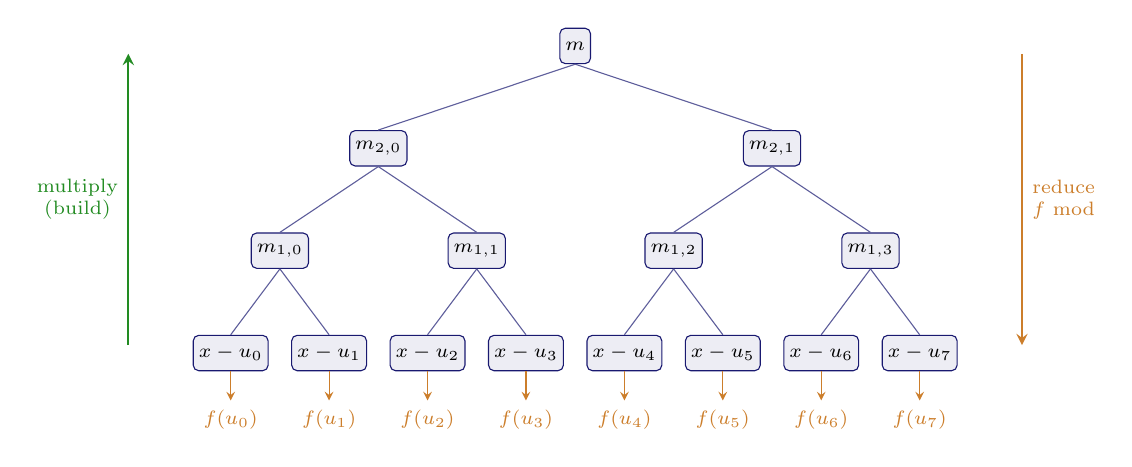
\begin{tikzpicture}[x=1cm,y=1cm,every node/.style={font=\scriptsize},>=stealth]
\tikzset{nd/.style={draw=MidnightBlue,fill=MidnightBlue!8,rounded corners=2pt,inner sep=2pt,minimum height=0.45cm}}
\node[nd] (n00) at (0.000,0.0) {$x-u_0$};
\node[nd] (n01) at (1.250,0.0) {$x-u_1$};
\node[nd] (n02) at (2.500,0.0) {$x-u_2$};
\node[nd] (n03) at (3.750,0.0) {$x-u_3$};
\node[nd] (n04) at (5.000,0.0) {$x-u_4$};
\node[nd] (n05) at (6.250,0.0) {$x-u_5$};
\node[nd] (n06) at (7.500,0.0) {$x-u_6$};
\node[nd] (n07) at (8.750,0.0) {$x-u_7$};
\node[nd] (n10) at (0.625,1.3) {$m_{1,0}$};
\draw[MidnightBlue!70] (n10.south) -- (n00.north);
\draw[MidnightBlue!70] (n10.south) -- (n01.north);
\node[nd] (n11) at (3.125,1.3) {$m_{1,1}$};
\draw[MidnightBlue!70] (n11.south) -- (n02.north);
\draw[MidnightBlue!70] (n11.south) -- (n03.north);
\node[nd] (n12) at (5.625,1.3) {$m_{1,2}$};
\draw[MidnightBlue!70] (n12.south) -- (n04.north);
\draw[MidnightBlue!70] (n12.south) -- (n05.north);
\node[nd] (n13) at (8.125,1.3) {$m_{1,3}$};
\draw[MidnightBlue!70] (n13.south) -- (n06.north);
\draw[MidnightBlue!70] (n13.south) -- (n07.north);
\node[nd] (n20) at (1.875,2.6) {$m_{2,0}$};
\draw[MidnightBlue!70] (n20.south) -- (n10.north);
\draw[MidnightBlue!70] (n20.south) -- (n11.north);
\node[nd] (n21) at (6.875,2.6) {$m_{2,1}$};
\draw[MidnightBlue!70] (n21.south) -- (n12.north);
\draw[MidnightBlue!70] (n21.south) -- (n13.north);
\node[nd] (n30) at (4.375,3.9000000000000004) {$m$};
\draw[MidnightBlue!70] (n30.south) -- (n20.north);
\draw[MidnightBlue!70] (n30.south) -- (n21.north);
\node[BurntOrange!80!black] (v0) at (0.000,-0.85) {$f(u_0)$};
\draw[->,BurntOrange!80!black] (n00.south) -- (v0.north);
\node[BurntOrange!80!black] (v1) at (1.250,-0.85) {$f(u_1)$};
\draw[->,BurntOrange!80!black] (n01.south) -- (v1.north);
\node[BurntOrange!80!black] (v2) at (2.500,-0.85) {$f(u_2)$};
\draw[->,BurntOrange!80!black] (n02.south) -- (v2.north);
\node[BurntOrange!80!black] (v3) at (3.750,-0.85) {$f(u_3)$};
\draw[->,BurntOrange!80!black] (n03.south) -- (v3.north);
\node[BurntOrange!80!black] (v4) at (5.000,-0.85) {$f(u_4)$};
\draw[->,BurntOrange!80!black] (n04.south) -- (v4.north);
\node[BurntOrange!80!black] (v5) at (6.250,-0.85) {$f(u_5)$};
\draw[->,BurntOrange!80!black] (n05.south) -- (v5.north);
\node[BurntOrange!80!black] (v6) at (7.500,-0.85) {$f(u_6)$};
\draw[->,BurntOrange!80!black] (n06.south) -- (v6.north);
\node[BurntOrange!80!black] (v7) at (8.750,-0.85) {$f(u_7)$};
\draw[->,BurntOrange!80!black] (n07.south) -- (v7.north);
\draw[->,thick,ForestGreen] (-1.3,0.1) -- (-1.3,3.8) node[midway,left,align=center] {multiply\\(build)};
\draw[->,thick,BurntOrange!80!black] (10.050,3.8) -- (10.050,0.1) node[midway,right,align=center] {reduce\\$f$ mod};
\end{tikzpicture}
